\documentclass[11pt,a4paper,oneside]{book}

% ------------------------------------------------------------------
%  Codificação e idioma
% ------------------------------------------------------------------
\usepackage[utf8]{inputenc}
\usepackage[T1]{fontenc}
\usepackage[brazil]{babel}
\usepackage{lmodern}

% ------------------------------------------------------------------
%  Matemática
% ------------------------------------------------------------------
\usepackage{amsmath,amssymb,amsthm,mathtools}
\usepackage{bm}

% ------------------------------------------------------------------
%  Figuras, tabelas e layout
% ------------------------------------------------------------------
\usepackage{graphicx}
% Busca as figuras primeiro na subpasta local "figs/" (cópia autocontida) e,
% caso não exista, nas pastas de imagens compartilhadas dos slides — mesma
% convenção usada pelos slides da disciplina (../images).
\graphicspath{{figs/}{../images/}{../../images/}}
\usepackage{float}
\usepackage{booktabs}
\usepackage{array}
\usepackage{caption}
\usepackage{subcaption}
\captionsetup{font=small,labelfont=bf}
\usepackage[dvipsnames,table]{xcolor}
\usepackage[a4paper,margin=2.7cm,headheight=14pt]{geometry}
\usepackage{microtype}
\usepackage{enumitem}
\usepackage{listings}
\usepackage{fancyhdr}
\usepackage{emptypage}

% ------------------------------------------------------------------
%  Hyperref (por último)
% ------------------------------------------------------------------
\usepackage[hidelinks,colorlinks=true,linkcolor=MidnightBlue,
            citecolor=MidnightBlue,urlcolor=RoyalBlue]{hyperref}

% ------------------------------------------------------------------
%  Cores do livro
% ------------------------------------------------------------------
\definecolor{corcap}{RGB}{20,60,110}
\definecolor{corbox}{RGB}{240,244,250}
\definecolor{corboxb}{RGB}{20,60,110}
\definecolor{corcode}{RGB}{248,248,248}

% ------------------------------------------------------------------
%  Ambientes de teorema (notação formal)
% ------------------------------------------------------------------
\theoremstyle{definition}
\newtheorem{definicao}{Definição}[chapter]
\newtheorem{exemplo}{Exemplo}[chapter]
\newtheorem{observacao}{Observação}[chapter]

\theoremstyle{plain}
\newtheorem{teorema}{Teorema}[chapter]
\newtheorem{proposicao}{Proposição}[chapter]
\newtheorem{corolario}{Corolário}[chapter]
\newtheorem{lema}{Lema}[chapter]

\renewcommand{\qedsymbol}{$\blacksquare$}

% Caixa de destaque para resultados-chave
\usepackage[most]{tcolorbox}
\usepackage{empheq}
\newtcolorbox{destaque}[1][]{
  colback=corbox, colframe=corboxb, boxrule=0.6pt, arc=2pt,
  left=6pt,right=6pt,top=5pt,bottom=5pt, #1}

% --- Caixas de destaque para os ambientes de teorema ---
\definecolor{corplain}{RGB}{20,60,110}   % azul (teorema/proposição/...)
\definecolor{cordef}{RGB}{110,80,20}     % âmbar (definição/exemplo/...)
\tcbset{
  thmplain/.style={breakable, enhanced, arc=2pt, boxrule=0.4pt,
    colback=corplain!5, colframe=corplain, left=8pt, right=8pt,
    top=5pt, bottom=5pt, borderline west={2.5pt}{0pt}{corplain}},
  thmdef/.style={breakable, enhanced, arc=2pt, boxrule=0.4pt,
    colback=cordef!6, colframe=cordef!85!black, left=8pt, right=8pt,
    top=5pt, bottom=5pt, borderline west={2.5pt}{0pt}{cordef!85!black}},
}
\tcolorboxenvironment{teorema}{thmplain}
\tcolorboxenvironment{proposicao}{thmplain}
\tcolorboxenvironment{corolario}{thmplain}
\tcolorboxenvironment{lema}{thmplain}
\tcolorboxenvironment{definicao}{thmdef}
\tcolorboxenvironment{exemplo}{thmdef}
\tcolorboxenvironment{observacao}{thmdef}

% --- Caixa para equações principais ---
% Uso: \begin{empheq}[box=\tcbhighmath]{equation} ... \end{empheq}
\tcbset{highlight math style={enhanced, colback=corplain!7,
  colframe=corplain, boxrule=0.5pt, arc=2pt,
  left=3pt, right=3pt, top=2pt, bottom=2pt}}

% ------------------------------------------------------------------
%  Cabeçalhos
% ------------------------------------------------------------------
\pagestyle{fancy}
\fancyhf{}
\renewcommand{\headrulewidth}{0.4pt}
\fancyhead[L]{\small\itshape SEL0359 -- Controle Digital}
\fancyhead[R]{\small\itshape\nouppercase{\leftmark}}
\fancyfoot[C]{\thepage}

% ------------------------------------------------------------------
%  Estilo de código
% ------------------------------------------------------------------
\lstdefinestyle{codigo}{
  backgroundcolor=\color{corcode},
  basicstyle=\ttfamily\small,
  keywordstyle=\color{MidnightBlue}\bfseries,
  commentstyle=\color{ForestGreen}\itshape,
  stringstyle=\color{BrickRed},
  numbers=left, numberstyle=\tiny\color{gray}, numbersep=8pt,
  frame=single, rulecolor=\color{gray!40},
  breaklines=true, showstringspaces=false, tabsize=2
}

% ------------------------------------------------------------------
%  Comandos utilitários
% ------------------------------------------------------------------
\newcommand{\Ztr}{\mathcal{Z}}
\newcommand{\Ltr}{\mathcal{L}}
\newcommand{\wn}{\omega_n}
\newcommand{\Real}{\operatorname{Re}}
\newcommand{\Imag}{\operatorname{Im}}
\DeclareMathOperator{\arctantwo}{atan2}

\allowdisplaybreaks

% ==================================================================
\begin{document}
% ==================================================================

\frontmatter

\begin{titlepage}
\centering
\vspace*{1.5cm}
{\Large\scshape Universidade de São Paulo\par}
{\large Escola de Engenharia de São Carlos\par}
{\large Departamento de Engenharia Elétrica e de Computação\par}
\vspace{1.2cm}
{\large\bfseries SEL0359 -- Controle Digital\par}
\vspace{2.2cm}
\rule{\linewidth}{0.5pt}\\[0.5cm]
{\Huge\bfseries Análise de Estabilidade\\[0.2cm] em Tempo Discreto\par}
\vspace{0.5cm}
{\large Transformada $z$, mapeamento $s\to z$, efeito da discretização\\
e o critério de Jury\par}
\rule{\linewidth}{0.5pt}\\[0.5cm]
\vspace{1.0cm}
{\large\itshape Apostila -- Aula 4\par}
\vfill
{\large Prof. Marcos Rogério Fernandes\par}
\vspace{0.5cm}
{\normalsize São Carlos, 2026\par}
\end{titlepage}

\tableofcontents
\cleardoublepage

\mainmatter

\chapter{Análise de Estabilidade em Tempo Discreto}
\label{cap:estabilidade}

\section{Introdução}

Um sistema de controle só é útil se for \emph{estável}. Antes de projetar
controladores (assunto do próximo capítulo), é indispensável dispor de
ferramentas que decidam se um dado sistema em malha fechada é estável e que
revelem \emph{como} a etapa de discretização afeta essa estabilidade. Este
capítulo constrói essas ferramentas para sistemas em tempo discreto.

\begin{figure}[H]
    \centering
    
\includegraphics[width=0.6\linewidth]{design_process.png}
    \caption[Ciclo do projeto de controle]{Ciclo de projeto de um sistema de
    controle. A análise de estabilidade é o alicerce sobre o qual todo o projeto
    se apoia: um controlador que desestabiliza a planta é inaceitável,
    independentemente de qualquer outro critério de desempenho.}
    \label{fig:ciclo}
\end{figure}

\begin{destaque}
\textbf{Objetivos do capítulo.} Ao final, o leitor deverá ser capaz de:
\begin{itemize}[nosep]
    \item deduzir a \textbf{transformada $z$} a partir da amostragem e
    manipular suas propriedades fundamentais;
    \item compreender o \textbf{mapeamento $s\to z$}, $z=e^{sT}$, e localizar a
    região de estabilidade no plano $z$;
    \item analisar o \textbf{efeito da discretização} (Euler e Tustin) sobre a
    região de estabilidade e o fenômeno da \textbf{distorção de frequência};
    \item aplicar o \textbf{critério de Jury} para decidir estabilidade sem
    calcular raízes;
    \item usar o \textbf{mapeamento bilinear no plano $w$} para reduzir o
    problema ao critério de Routh--Hurwitz.
\end{itemize}
\end{destaque}

\section{Sinais em tempo discreto e a transformada \texorpdfstring{$z$}{z}}
\label{sec:ztransform}

\subsection{Sinal em tempo discreto e sinal amostrado}

\begin{definicao}[Sinal em tempo discreto]
Um \textbf{sinal em tempo discreto} é uma sequência obtida pela amostragem
uniforme de um sinal contínuo $x(t)$ a cada período $T$:
\begin{equation}
    x[k]=x(kT),\qquad k\in\mathbb{Z}.
    \label{eq:xk}
\end{equation}
\end{definicao}

\begin{figure}[H]
    \centering
    
\includegraphics[width=0.55\linewidth]{sequencia_sinal.png}
    \caption[Sequência discreta]{Sinal em tempo discreto $x[k]=x(kT)$: uma
    sequência de amostras indexadas pelo inteiro $k$.}
    \label{fig:seq}
\end{figure}

Para conectar o mundo discreto ao contínuo, modela-se a amostragem por um trem de
impulsos ponderados pelas amostras.

\begin{definicao}[Sinal amostrado idealmente]
O \textbf{sinal amostrado} associado a $x(t)$ é
\begin{equation}
    x_a^*(t)=\sum_{k=-\infty}^{\infty}x(kT)\,\delta(t-kT),
    \label{eq:xa}
\end{equation}
em que $\delta(\cdot)$ é o impulso de Dirac.
\end{definicao}

\begin{figure}[H]
    \centering
    
\includegraphics[width=0.5\linewidth]{modular_amostragem2.png}
    \caption[Amostragem por trem de impulsos]{Interpretação da amostragem como
    modulação de um trem de impulsos: cada impulso, no instante $kT$, carrega o
    peso $x(kT)$.}
    \label{fig:amostragem}
\end{figure}

\subsection{Da transformada de Laplace à transformada \texorpdfstring{$z$}{z}}

Aplicar a transformada de Laplace ao sinal amostrado \eqref{eq:xa} revela
naturalmente a variável $z$.

\begin{proposicao}[Laplace do sinal amostrado]
\label{prop:laplace}
A transformada de Laplace de $x_a^*(t)$ é
\begin{equation}
    \Ltr\{x_a^*(t)\}=\sum_{k=-\infty}^{\infty}x[k]\,\big(e^{sT}\big)^{-k}.
    \label{eq:laplace_amostrado}
\end{equation}
\end{proposicao}

\begin{proof}
Por definição da transformada de Laplace e de \eqref{eq:xa},
\[
\Ltr\{x_a^*(t)\}
=\int_{-\infty}^{\infty}\Bigg(\sum_{k=-\infty}^{\infty}x(kT)\,\delta(t-kT)\Bigg)e^{-st}\,dt.
\]
Trocando a ordem entre soma e integral (linearidade),
\[
=\sum_{k=-\infty}^{\infty}x(kT)\int_{-\infty}^{\infty}\delta(t-kT)\,e^{-st}\,dt.
\]
Pela propriedade de amostragem (\emph{sifting}) do impulso,
$\int_{-\infty}^{\infty}\delta(t-kT)e^{-st}\,dt=e^{-skT}$, logo
\[
\Ltr\{x_a^*(t)\}=\sum_{k=-\infty}^{\infty}x(kT)\,e^{-skT}
              =\sum_{k=-\infty}^{\infty}x[k]\,\big(e^{sT}\big)^{-k}.
\]
\end{proof}

A Proposição~\ref{prop:laplace} mostra que $s$ aparece somente através da
combinação $e^{sT}$. Isso motiva a mudança de variável central de todo o curso.

\begin{destaque}
\textbf{Definição da variável $z$.} Define-se
\begin{equation}
    \boxed{\,z=e^{sT}\,}
    \label{eq:zdef}
\end{equation}
Com essa substituição, a soma \eqref{eq:laplace_amostrado} torna-se a
\emph{transformada $z$} da sequência $x[k]$.
\end{destaque}

\begin{definicao}[Transformada $z$]
\label{def:z}
Dada uma função $x:\mathbb{Z}\to\mathbb{C}$, a \textbf{transformada $z$} de
$x[k]$ é o mapeamento $X:\mathcal{D}\to\mathbb{C}$ definido por
\begin{equation}
    \Ztr\{x[k]\}=\sum_{k=-\infty}^{\infty}x[k]\,z^{-k}=X(z),
    \label{eq:ztransform}
\end{equation}
em que o domínio $\mathcal{D}\subseteq\mathbb{C}$, chamado \textbf{região de
convergência} (ROC), é o conjunto
\begin{equation}
    \mathcal{D}=\{z\in\mathbb{C}:X(z)\ \text{existe (a série converge)}\}.
    \label{eq:roc}
\end{equation}
\end{definicao}

\subsection{Série geométrica e região de convergência}

A convergência da série \eqref{eq:ztransform} apoia-se na série geométrica.

\begin{lema}[Série geométrica]
\label{lema:geom}
Seja $z\in\mathbb{C}$. Se $|z|<1$, então
\begin{equation}
    \sum_{k=0}^{\infty}z^{k}=\frac{1}{1-z}.
    \label{eq:geom}
\end{equation}
\end{lema}

\begin{proof}
Seja $S_N=\sum_{k=0}^{N}z^k$ a soma parcial. Então
$(1-z)S_N=S_N-zS_N=1-z^{N+1}$, de modo que, para $z\neq 1$,
$S_N=\frac{1-z^{N+1}}{1-z}$. Se $|z|<1$, então $|z^{N+1}|=|z|^{N+1}\to 0$ quando
$N\to\infty$, e portanto $S_N\to\frac{1}{1-z}$, o que prova \eqref{eq:geom}.
\end{proof}

\begin{observacao}
A condição $|z|<1$ é exatamente uma restrição sobre a \emph{região de
convergência}. Para uma sequência causal do tipo $x[k]=a^k u[k]$, por exemplo, a
série converge para $|z|>|a|$ --- o exterior de um círculo. A
Figura~\ref{fig:roc} ilustra uma ROC típica no plano $z$.
\end{observacao}

\begin{figure}[H]
    \centering
    
\includegraphics[width=0.5\linewidth]{ROC_ztrans.png}
    \caption[Região de convergência]{Região de convergência (ROC) no plano $z$.
    A transformada $z$ só está definida onde a série que a define converge; a
    fronteira é sempre um círculo centrado na origem.}
    \label{fig:roc}
\end{figure}

\subsection{Propriedade do deslocamento (atraso)}

A propriedade que torna a transformada $z$ a ferramenta natural para equações a
diferenças é a do deslocamento temporal.

\begin{proposicao}[Deslocamento no tempo]
\label{prop:shift}
Seja $X(z)=\Ztr\{x[k]\}$. Então, para todo inteiro $m$,
\begin{equation}
    \Ztr\{x[k-m]\}=z^{-m}X(z).
    \label{eq:shift}
\end{equation}
\end{proposicao}

\begin{proof}
Por definição, $\Ztr\{x[k-m]\}=\sum_{k=-\infty}^{\infty}x[k-m]z^{-k}$. Fazendo a
mudança de índice $n=k-m$ (logo $k=n+m$),
\[
\Ztr\{x[k-m]\}=\sum_{n=-\infty}^{\infty}x[n]\,z^{-(n+m)}
=z^{-m}\sum_{n=-\infty}^{\infty}x[n]\,z^{-n}=z^{-m}X(z).
\]
\end{proof}

Um atraso de $m$ amostras no tempo corresponde, portanto, à multiplicação por
$z^{-m}$ no domínio transformado --- é por isso que $z^{-1}$ é o ``operador de
atraso unitário''.

\subsection{Equações a diferenças e função de transferência}

\begin{exemplo}[Da equação a diferenças à função de transferência]
\label{ex:edo}
Considere o sistema discreto (Figura~\ref{fig:sistema}) descrito pela equação a
diferenças
\begin{equation}
    y[k]=a_1 y[k-1]+a_2 y[k-2]+u[k]+b_1 u[k-1].
    \label{eq:edo}
\end{equation}
Obtenha a função de transferência $G(z)=Y(z)/U(z)$.
\end{exemplo}

\begin{figure}[H]
    \centering
    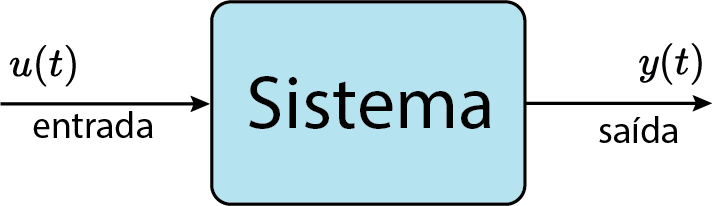
\includegraphics[width=0.32\linewidth]{sistema.png}
    \caption[Sistema entrada--saída]{Sistema discreto com entrada $u[k]$ e saída
    $y[k]$, caracterizado por sua função de transferência $G(z)$.}
    \label{fig:sistema}
\end{figure}

\noindent\textbf{Solução.} Aplicando a transformada $z$ a \eqref{eq:edo} e usando
a propriedade do deslocamento (Proposição~\ref{prop:shift}),
\[
Y(z)=a_1 z^{-1}Y(z)+a_2 z^{-2}Y(z)+U(z)+b_1 z^{-1}U(z).
\]
Agrupando os termos em $Y(z)$ de um lado e em $U(z)$ do outro,
\[
\big(1-a_1 z^{-1}-a_2 z^{-2}\big)Y(z)=\big(1+b_1 z^{-1}\big)U(z),
\]
de onde
\begin{empheq}[box=\tcbhighmath]{equation}
    \frac{Y(z)}{U(z)}=\frac{1+b_1 z^{-1}}{1-a_1 z^{-1}-a_2 z^{-2}}=G(z).
    \label{eq:Gz}
\end{empheq}
Multiplicando numerador e denominador por $z^2$, obtém-se a forma em potências
positivas $G(z)=\dfrac{z^2+b_1 z}{z^2-a_1 z-a_2}$, cujas raízes do denominador são
os \emph{polos} do sistema --- objeto central da análise de estabilidade.

\section{Mapeamento do plano \texorpdfstring{$s$}{s} no plano \texorpdfstring{$z$}{z}}
\label{sec:mapeamento}

A relação $z=e^{sT}$ (Eq.~\eqref{eq:zdef}) é uma função que leva cada ponto do
plano complexo $s$ a um ponto do plano complexo $z$. Compreender essa
transformação é a chave para transportar a noção de estabilidade do tempo
contínuo (bem conhecida) para o tempo discreto.

\begin{figure}[H]
    \centering
    
\includegraphics[width=0.85\linewidth]{plano_s_plano_z.png}
    \caption[Mapeamento $s\to z$]{Mapeamento do plano $s$ (esquerda) no plano
    $z$ (direita) pela relação $z=e^{sT}$. Regiões inteiras do plano $s$ são
    ``enroladas'' em torno da origem do plano $z$.}
    \label{fig:map_sz}
\end{figure}

\subsection{Decomposição do mapeamento}

\begin{proposicao}[Módulo e fase da imagem]
\label{prop:modfase}
Seja $s=\sigma+j\omega$. Então
\begin{equation}
    z=e^{sT}=e^{(\sigma+j\omega)T}=\underbrace{e^{\sigma T}}_{|z|}\;
             \underbrace{e^{j\omega T}}_{\angle z},
    \label{eq:modfase}
\end{equation}
isto é, $|z|=e^{\sigma T}$ e $\angle z=\omega T$.
\end{proposicao}

\begin{proof}
Basta separar a parte real e imaginária no expoente:
$e^{(\sigma+j\omega)T}=e^{\sigma T}\,e^{j\omega T}$. Como $e^{\sigma T}>0$ é real e
$|e^{j\omega T}|=1$, tem-se $|z|=e^{\sigma T}$ e $\angle z=\omega T$.
\end{proof}

A Proposição~\ref{prop:modfase} tem uma leitura geométrica direta: a
\emph{parte real} $\sigma$ de $s$ controla o \emph{módulo} de $z$, enquanto a
\emph{parte imaginária} $\omega$ controla o \emph{ângulo} de $z$. Analisemos as
retas verticais $\sigma=\text{constante}$.

\begin{corolario}[Imagem das retas verticais]
\label{cor:retas}
A reta vertical $\{s=\sigma_0+j\omega:\omega\in\mathbb{R}\}$ é mapeada no círculo
de raio $e^{\sigma_0 T}$ centrado na origem do plano $z$. Em particular:
\begin{itemize}[nosep]
    \item $\sigma_0=0$ (eixo imaginário) $\mapsto$ círculo de raio $1$ (círculo
    unitário);
    \item $\sigma_0<0$ (semiplano esquerdo) $\mapsto$ círculo de raio $<1$
    (interior do círculo unitário);
    \item $\sigma_0>0$ (semiplano direito) $\mapsto$ círculo de raio $>1$
    (exterior do círculo unitário).
\end{itemize}
\end{corolario}

\begin{proof}
Pela Proposição~\ref{prop:modfase}, ao longo da reta $\sigma=\sigma_0$ tem-se
$|z|=e^{\sigma_0 T}$ constante, enquanto $\angle z=\omega T$ percorre todos os
valores quando $\omega$ varia em $\mathbb{R}$. Logo a imagem é o círculo
$|z|=e^{\sigma_0 T}$. O sinal de $\sigma_0$ determina se $e^{\sigma_0 T}$ é menor,
igual ou maior que $1$.
\end{proof}

As Figuras~\ref{fig:map_lines} ilustram esse enrolamento para $\sigma=0$,
$\sigma<0$ e $\sigma>0$.

\begin{figure}[H]
    \centering
    \begin{subfigure}{\linewidth}
        \centering
        
\includegraphics[width=0.9\linewidth]{map0.png}
        \caption{$\sigma=0$: o eixo imaginário mapeia-se \emph{sobre} o círculo
        unitário.}
    \end{subfigure}\\[4pt]
    \begin{subfigure}{0.49\linewidth}
        \centering
        
\includegraphics[width=\linewidth]{map3.png}
        \caption{$\sigma=-0{,}3$: reta no SPE $\mapsto$ círculo \emph{interno}.}
    \end{subfigure}\hfill
    \begin{subfigure}{0.49\linewidth}
        \centering
        
\includegraphics[width=\linewidth]{map_pos3.png}
        \caption{$\sigma=+0{,}3$: reta no SPD $\mapsto$ círculo \emph{externo}.}
    \end{subfigure}
    \caption[Imagem das retas verticais]{Imagem de retas verticais do plano $s$
    sob $z=e^{sT}$. O semiplano esquerdo (SPE) é comprimido para dentro do
    círculo unitário; o eixo imaginário vai para a circunferência; o semiplano
    direito (SPD) vai para fora.}
    \label{fig:map_lines}
\end{figure}

Reunindo as três regiões, obtém-se o resultado fundamental deste capítulo.

\begin{teorema}[Mapeamento da região de estabilidade]
\label{teo:regiao}
O mapeamento $z=e^{sT}$ leva o semiplano esquerdo aberto do plano $s$
($\Real\{s\}<0$) para o interior do círculo unitário do plano $z$ ($|z|<1$); o
eixo imaginário ($\Real\{s\}=0$) para a circunferência unitária ($|z|=1$); e o
semiplano direito ($\Real\{s\}>0$) para o exterior ($|z|>1$).
\end{teorema}

\begin{proof}
Para $s=\sigma+j\omega$, a Proposição~\ref{prop:modfase} fornece $|z|=e^{\sigma
T}$ com $T>0$. A função $\sigma\mapsto e^{\sigma T}$ é estritamente crescente e
satisfaz $e^{\sigma T}<1\iff\sigma<0$, $e^{\sigma T}=1\iff\sigma=0$ e
$e^{\sigma T}>1\iff\sigma>0$. Como a condição sobre $|z|$ depende apenas de
$\sigma=\Real\{s\}$, as três equivalências correspondem exatamente às três
regiões enunciadas.
\end{proof}

\begin{figure}[H]
    \centering
    \begin{subfigure}{0.31\linewidth}
        \centering
        
\includegraphics[width=\linewidth]{plano_s_plano_z_SPE.png}
        \caption{SPE $\to$ interior.}
    \end{subfigure}\hfill
    \begin{subfigure}{0.31\linewidth}
        \centering
        
\includegraphics[width=\linewidth]{plano_s_plano_z_jw.png}
        \caption{Eixo $j\omega\to$ círculo.}
    \end{subfigure}\hfill
    \begin{subfigure}{0.31\linewidth}
        \centering
        
\includegraphics[width=\linewidth]{plano_s_plano_z_SPD.png}
        \caption{SPD $\to$ exterior.}
    \end{subfigure}
    \caption[Regiões do mapeamento]{Correspondência entre as regiões de
    estabilidade do plano $s$ e do plano $z$ sob $z=e^{sT}$
    (Teorema~\ref{teo:regiao}).}
    \label{fig:regioes}
\end{figure}

\begin{observacao}[Faixa principal e aliasing]
Como $e^{j\omega T}$ é periódico em $\omega$ com período $\omega_s=2\pi/T$, todas
as faixas horizontais de altura $\omega_s$ no plano $s$ têm a \emph{mesma} imagem
no plano $z$. A faixa $-\omega_s/2<\omega\le\omega_s/2$ é chamada \textbf{faixa
principal}; as demais são réplicas. Essa periodicidade é a manifestação, no
plano complexo, do fenômeno de \emph{aliasing}.
\end{observacao}

\begin{figure}[H]
    \centering
    
\includegraphics[width=0.85\linewidth]{plano_s_plano_z_faixa_princ.png}
    \caption[Faixa principal]{Faixa principal do plano $s$ (esquerda) e sua
    imagem no plano $z$ (direita). Faixas deslocadas de múltiplos de
    $\omega_s=2\pi/T$ recaem sobre a mesma região do plano $z$.}
    \label{fig:faixa}
\end{figure}

\subsection{Mapeamento dos polos dominantes de segunda ordem}

Um caso de especial importância prática é o dos polos de um sistema de segunda
ordem subamortecido,
\begin{empheq}[box=\tcbhighmath]{equation}
    G(s)=\frac{\wn^2}{s^2+2\xi\wn s+\wn^2},\qquad 0\le\xi<1,
    \label{eq:2ordem}
\end{empheq}
cujos polos, no plano $s$, são
\begin{equation}
    p_{1,2}=-\xi\wn\pm j\wn\sqrt{1-\xi^2}.
    \label{eq:polos_s}
\end{equation}

\begin{proposicao}[Imagem dos polos de segunda ordem]
\label{prop:polos_z}
Sob $z=e^{sT}$, os polos \eqref{eq:polos_s} são mapeados em
\begin{equation}
    p_{1,2}^{z}=e^{-\xi\wn T}\,e^{\pm j\wn T\sqrt{1-\xi^2}}.
    \label{eq:polos_z}
\end{equation}
\end{proposicao}

\begin{proof}
Aplicação direta de $z=e^{sT}$ a \eqref{eq:polos_s}, separando módulo
($e^{-\xi\wn T}$) e fase ($\pm\wn T\sqrt{1-\xi^2}$), como na
Proposição~\ref{prop:modfase}.
\end{proof}

As Figuras~\ref{fig:2nd_xi} e \ref{fig:2nd_wn} mostram como a posição no plano
$z$ varia ao percorrer, respectivamente, o amortecimento $\xi$ e a frequência
natural $\wn$; a resposta ao degrau correspondente aparece na
Figura~\ref{fig:subam}.

\begin{figure}[H]
    \centering
    \begin{subfigure}{0.49\linewidth}
        \centering
\includegraphics[width=\linewidth]{subamortecido_step.png}
        \caption{$\wn=1$ fixo, variando $\xi$.}
    \end{subfigure}\hfill
    \begin{subfigure}{0.49\linewidth}
        \centering
\includegraphics[width=\linewidth]{subamortecido_step_wn.png}
        \caption{$\xi=0{,}2$ fixo, variando $\wn$.}
    \end{subfigure}
    \caption[Respostas ao degrau de 2ª ordem]{Respostas ao degrau do sistema
    subamortecido. Menor $\xi$ aumenta o sobressinal; maior $\wn$ acelera a
    resposta.}
    \label{fig:subam}
\end{figure}

\begin{figure}[H]
    \centering
    \begin{subfigure}{0.32\linewidth}
        \centering
\includegraphics[width=\linewidth]{2nd_pole_xi3.png}
        \caption{$\xi=0{,}3$.}
    \end{subfigure}\hfill
    \begin{subfigure}{0.32\linewidth}
        \centering
\includegraphics[width=\linewidth]{2nd_pole_xi6.png}
        \caption{$\xi=0{,}6$.}
    \end{subfigure}\hfill
    \begin{subfigure}{0.32\linewidth}
        \centering
\includegraphics[width=\linewidth]{2nd_pole_xi9.png}
        \caption{$\xi=0{,}9$.}
    \end{subfigure}
    \caption[Variação de $\xi$]{Posição dos polos no plano $s$ e no plano $z$ ao
    variar o amortecimento $\xi$ (com $\wn$ fixo).}
    \label{fig:2nd_xi}
\end{figure}

\begin{figure}[H]
    \centering
    \begin{subfigure}{0.32\linewidth}
        \centering
\includegraphics[width=\linewidth]{2nd_pole_wn1.png}
        \caption{$\wn=0{,}3$ rad/s.}
    \end{subfigure}\hfill
    \begin{subfigure}{0.32\linewidth}
        \centering
\includegraphics[width=\linewidth]{2nd_pole_wn5.png}
        \caption{$\wn=1{,}1$ rad/s.}
    \end{subfigure}\hfill
    \begin{subfigure}{0.32\linewidth}
        \centering
\includegraphics[width=\linewidth]{2nd_pole_wn10.png}
        \caption{$\wn=2{,}1$ rad/s.}
    \end{subfigure}
    \caption[Variação de $\wn$]{Posição dos polos no plano $s$ e no plano $z$ ao
    variar a frequência natural $\wn$ (com $\xi$ fixo).}
    \label{fig:2nd_wn}
\end{figure}

O lugar geométrico de $\xi$ e $\wn$ constantes, mapeado para o plano $z$, é a
conhecida \emph{$z$-grid} (Figura~\ref{fig:zgrid}), ferramenta gráfica para
posicionar polos discretos segundo especificações de desempenho.

\begin{figure}[H]
    \centering
    \begin{subfigure}{0.5\linewidth}
        \centering
\includegraphics[width=\linewidth]{zgrid00.png}
        \caption{$z$-grid completa.}
    \end{subfigure}\hfill
    \begin{subfigure}{0.24\linewidth}
        \centering
\includegraphics[width=\linewidth]{zgrid02.png}
        \caption{$\xi=0{,}2$.}
    \end{subfigure}\hfill
    \begin{subfigure}{0.24\linewidth}
        \centering
\includegraphics[width=\linewidth]{zgrid_wn.png}
        \caption{$\wn$ const.}
    \end{subfigure}
    \caption[$z$-grid]{Curvas de $\xi$ e $\wn$ constantes mapeadas para o plano
    $z$. Retas de $\xi$ constante tornam-se espirais logarítmicas; círculos de
    $\wn$ constante tornam-se curvas fechadas.}
    \label{fig:zgrid}
\end{figure}

\section{Estabilidade em malha fechada}
\label{sec:malha}

\subsection{Do contínuo ao discreto}

Recordemos o critério de estabilidade em tempo contínuo. Para a malha fechada
com realimentação unitária da Figura~\ref{fig:mf_s},
\begin{equation}
    G_f(s)=\frac{G(s)}{1+G(s)},\qquad P(s)=1+G(s),
\end{equation}
o sistema é assintoticamente estável se e somente se todas as raízes da
\emph{equação característica} $P(s)=0$ estão no semiplano esquerdo (SPE), isto é,
possuem parte real negativa.

\begin{figure}[H]
    \centering
    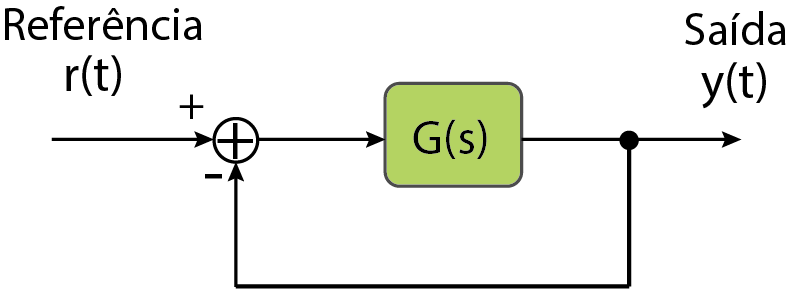
\includegraphics[width=0.55\linewidth]{malha_fechada_s.png}
    \caption[Malha fechada contínua]{Malha fechada em tempo contínuo com
    realimentação unitária. A estabilidade é decidida pelas raízes de
    $P(s)=1+G(s)$.}
    \label{fig:mf_s}
\end{figure}

\begin{figure}[H]
    \centering
    
\includegraphics[width=0.5\linewidth]{estabilidade_s.png}
    \caption[Região estável no plano $s$]{Região de estabilidade no plano $s$:
    semiplano esquerdo aberto ($\Real\{s\}<0$).}
    \label{fig:est_s}
\end{figure}

Pelo Teorema~\ref{teo:regiao}, o SPE mapeia-se no interior do círculo unitário.
Isso transporta imediatamente o critério para o tempo discreto.

\begin{definicao}[Estabilidade assintótica em tempo discreto]
\label{def:estavel}
A malha fechada discreta (Figura~\ref{fig:mf_z}), com
\begin{equation}
    G_f(z)=\frac{G(z)}{1+G(z)},\qquad Q(z)=1+G(z),
\end{equation}
é \textbf{assintoticamente estável} se e somente se todas as raízes da equação
característica $Q(z)=0$ estão no \emph{interior do círculo unitário}:
\begin{equation}
    Q(z_i)=0\ \Longrightarrow\ |z_i|<1.
\end{equation}
\end{definicao}

\begin{figure}[H]
    \centering
    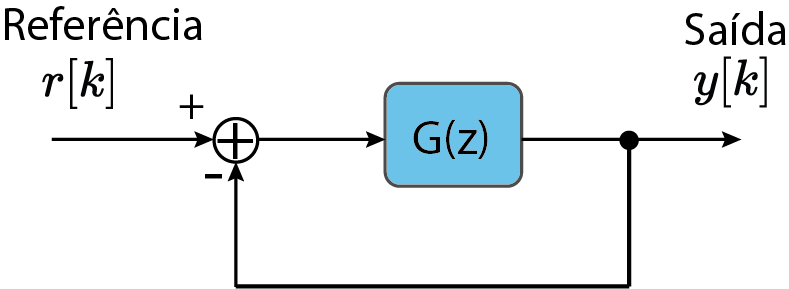
\includegraphics[width=0.55\linewidth]{malha_fechada_z.png}
    \caption[Malha fechada discreta]{Malha fechada em tempo discreto com
    realimentação unitária. A estabilidade é decidida pelas raízes de
    $Q(z)=1+G(z)$.}
    \label{fig:mf_z}
\end{figure}

\begin{figure}[H]
    \centering
    
\includegraphics[width=0.5\linewidth]{estabilidade_z.png}
    \caption[Região estável no plano $z$]{Região de estabilidade no plano $z$:
    interior do círculo unitário ($|z|<1$).}
    \label{fig:est_z}
\end{figure}

\section{Efeito da discretização na estabilidade}
\label{sec:discretizacao}

Quando um controlador (ou uma planta) projetado no contínuo é discretizado por um
método aproximado, a substituição de $s$ por uma função de $z$ \emph{deforma} a
região de estabilidade. A pergunta é: em que região do plano $z$ recai o
semiplano esquerdo ($\Real\{s\}<0$) sob cada método? Analisamos os três métodos
clássicos.

\subsection{Euler \emph{forward}}

\begin{proposicao}[Região de estabilidade --- Euler \emph{forward}]
\label{prop:forward}
No método de Euler \emph{forward}, $s=\dfrac{z-1}{T}$, a condição de estabilidade
contínua $\Real\{s\}<0$ corresponde, no plano $z$, ao semiplano
\begin{equation}
    \Real\{z\}<1.
\end{equation}
\end{proposicao}

\begin{proof}
Escreva $z=a+jb$. Então
\[
\Real\{s\}=\Real\!\left\{\frac{z-1}{T}\right\}
=\Real\!\left\{\frac{(a-1)+jb}{T}\right\}=\frac{a-1}{T}.
\]
Como $T>0$, a condição $\Real\{s\}<0$ equivale a $a-1<0$, ou seja, $a=\Real\{z\}<1$.
\end{proof}

\begin{figure}[H]
    \centering
    
\includegraphics[width=0.6\linewidth]{map_plano_s_euler_forwar.png}
    \caption[Euler \emph{forward}]{Imagem do semiplano esquerdo sob Euler
    \emph{forward}: o semiplano $\Real\{z\}<1$. Essa região \emph{contém} o
    círculo unitário, mas é muito maior: um sistema contínuo estável pode gerar
    um discreto instável (polos com $|z|>1$ e $\Real\{z\}<1$), sobretudo com
    período de amostragem $T$ grande.}
    \label{fig:forward}
\end{figure}

\subsection{Euler \emph{backward}}

\begin{proposicao}[Região de estabilidade --- Euler \emph{backward}]
\label{prop:backward}
No método de Euler \emph{backward}, $s=\dfrac{z-1}{zT}$, a condição
$\Real\{s\}<0$ corresponde ao \emph{disco}
\begin{equation}
    \left(a-\tfrac12\right)^2+b^2<\left(\tfrac12\right)^2,\qquad z=a+jb,
\end{equation}
isto é, o disco de centro $z=\tfrac12$ e raio $\tfrac12$.
\end{proposicao}

\begin{proof}
Com $z=a+jb$,
\[
\Real\{s\}=\Real\!\left\{\frac{a+jb-1}{(a+jb)T}\right\}.
\]
Multiplica-se numerador e denominador pelo conjugado $(a-jb)$ do denominador:
\[
\frac{(a-1+jb)(a-jb)}{(a^2+b^2)\,T}.
\]
O denominador é real e positivo, de modo que o sinal de $\Real\{s\}$ é o de
$\Real\{(a-1+jb)(a-jb)\}$. Expandindo,
\[
\Real\{(a-1+jb)(a-jb)\}=\Real\{(a^2+b^2)-(a-jb)\}=a^2+b^2-a.
\]
Logo $\Real\{s\}<0\iff a^2-a+b^2<0$. Completando o quadrado em $a$,
\[
\left(a-\tfrac12\right)^2-\tfrac14+b^2<0
\;\Longrightarrow\;
\left(a-\tfrac12\right)^2+b^2<\left(\tfrac12\right)^2.
\]
\end{proof}

\begin{figure}[H]
    \centering
    
\includegraphics[width=0.6\linewidth]{map_plano_s_euler_backward.png}
    \caption[Euler \emph{backward}]{Imagem do semiplano esquerdo sob Euler
    \emph{backward}: o disco de centro $\tfrac12$ e raio $\tfrac12$. Essa região
    está \emph{inteiramente contida} no círculo unitário, de modo que o método é
    sempre estável --- porém pode tornar estável um sistema que deveria ser
    instável, distorcendo o comportamento.}
    \label{fig:backward}
\end{figure}

\subsection{Bilinear (Tustin)}

\begin{teorema}[Região de estabilidade --- Tustin]
\label{teo:tustin}
No método bilinear (Tustin), $s=\dfrac{2}{T}\dfrac{z-1}{z+1}$, a condição
$\Real\{s\}<0$ corresponde \emph{exatamente} ao interior do círculo unitário,
\begin{equation}
    a^2+b^2<1,\qquad z=a+jb,
\end{equation}
isto é, $|z|<1$.
\end{teorema}

\begin{proof}
Com $z=a+jb$,
\[
\Real\{s\}=\Real\!\left\{\frac{2}{T}\frac{(a-1)+jb}{(a+1)+jb}\right\}.
\]
Multiplicando pelo conjugado $(a+1)-jb$ do denominador,
\[
\frac{2}{T}\cdot\frac{\big[(a-1)+jb\big]\big[(a+1)-jb\big]}{(a+1)^2+b^2}.
\]
O denominador é real e positivo. O numerador (parte real) é
\[
\Real\{[(a-1)+jb][(a+1)-jb]\}=(a-1)(a+1)+b^2=a^2-1+b^2.
\]
Assim, $\Real\{s\}<0\iff a^2+b^2-1<0\iff a^2+b^2<1$, isto é, $|z|<1$.
\end{proof}

\begin{figure}[H]
    \centering
    
\includegraphics[width=0.6\linewidth]{map_plano_s_tustin.png}
    \caption[Tustin]{Imagem do semiplano esquerdo sob Tustin: exatamente o
    interior do círculo unitário. O método bilinear é o único dos três que
    \emph{preserva a região de estabilidade} --- ele estabelece uma
    correspondência biunívoca entre SPE e disco unitário.}
    \label{fig:tustin}
\end{figure}

\begin{destaque}
\textbf{Comparação dos três métodos.}
\begin{itemize}[nosep]
    \item \textbf{Euler \emph{forward}} ($\Real\{z\}<1$): região maior que o
    disco unitário --- \emph{não} garante estabilidade do discreto;
    \item \textbf{Euler \emph{backward}} (disco de raio $\tfrac12$): região
    interna ao disco unitário --- sempre estável, mas conservador;
    \item \textbf{Tustin} ($|z|<1$): coincide com o disco unitário --- preserva
    exatamente a estabilidade.
\end{itemize}
Por isso Tustin é o método preferido para discretizar preservando estabilidade.
\end{destaque}

\subsection{Distorção de frequência (\emph{warping}) no método de Tustin}

Embora preserve a estabilidade, o método de Tustin distorce o eixo de
frequências. Vejamos como.

\begin{teorema}[Distorção de frequência]
\label{teo:warp}
Sob o método de Tustin, a frequência analógica $\omega$ e a frequência digital
$\omega_D$ (do sinal amostrado) relacionam-se por
\begin{equation}
    \omega=\frac{2}{T}\tan\!\left(\omega_D\,\frac{T}{2}\right).
    \label{eq:warp}
\end{equation}
\end{teorema}

\begin{proof}
Avaliamos a relação de Tustin sobre o eixo imaginário ($\sigma=0$), com
$z=e^{sT}\big|_{\sigma=0}=e^{j\omega_D T}$:
\[
j\omega=\frac{2}{T}\frac{e^{j\omega_D T}-1}{e^{j\omega_D T}+1}.
\]
Multiplicando numerador e denominador por $e^{-j\omega_D T/2}$,
\[
j\omega=\frac{2}{T}\frac{e^{j\omega_D T/2}-e^{-j\omega_D T/2}}
                        {e^{j\omega_D T/2}+e^{-j\omega_D T/2}}.
\]
Pelas fórmulas de Euler, $e^{j\theta}-e^{-j\theta}=2j\sin\theta$ e
$e^{j\theta}+e^{-j\theta}=2\cos\theta$ com $\theta=\omega_D T/2$:
\[
j\omega=\frac{2}{T}\frac{2j\sin(\omega_D T/2)}{2\cos(\omega_D T/2)}
       =j\,\frac{2}{T}\tan\!\left(\omega_D\frac{T}{2}\right).
\]
Cancelando $j$, obtém-se \eqref{eq:warp}.
\end{proof}

\begin{corolario}[Regime de alta taxa de amostragem]
Para $\omega_D T/2\ll 1$, vale $\tan(\omega_D T/2)\approx\omega_D T/2$ e,
portanto, $\omega\approx\omega_D$: a distorção é desprezível quando a frequência
de amostragem é muito maior que as frequências de interesse.
\end{corolario}

\begin{figure}[H]
    \centering
    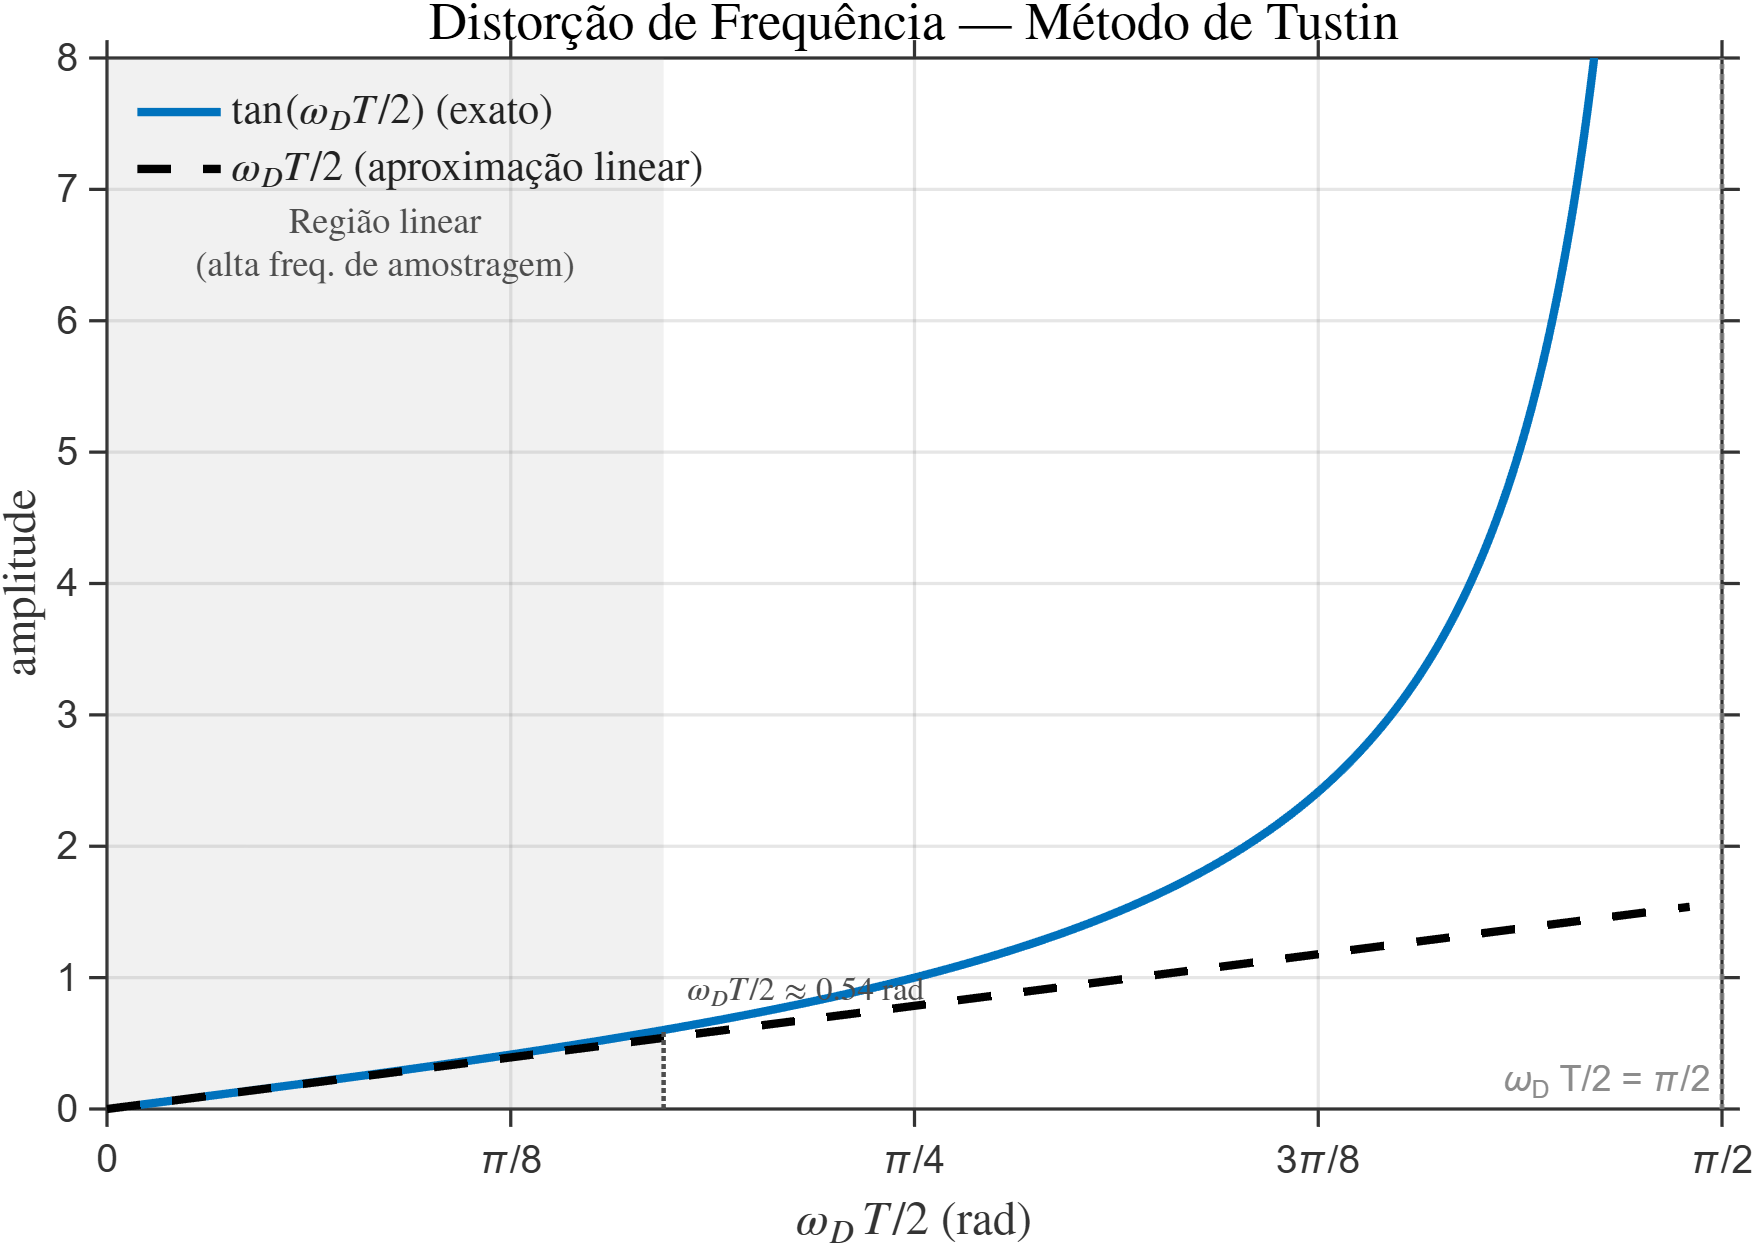
\includegraphics[width=0.5\linewidth]{distorcao_frequencia_tustin.png}
    \caption[\emph{Warping} de frequência]{Relação não linear entre a frequência
    analógica $\omega$ e a digital $\omega_D$ no método de Tustin. Próximo à
    origem a relação é praticamente linear ($\omega\approx\omega_D$); perto da
    frequência de Nyquist ela ``comprime'' fortemente o eixo.}
    \label{fig:warp}
\end{figure}

\subsection{\emph{Prewarping}}

Para que a discretização por Tustin case \emph{exatamente} em uma frequência
crítica $\omega_c$ (por exemplo, uma frequência de corte), pré-distorce-se a
transformação.

\begin{proposicao}[\emph{Prewarping}]
Para cancelar a distorção na frequência $\omega_c$, utiliza-se a substituição
modificada
\begin{equation}
    s:=\frac{\omega_c}{\tan\!\left(\omega_c\,\frac{T}{2}\right)}\,\frac{z-1}{z+1}.
    \label{eq:prewarp}
\end{equation}
No MATLAB, isso corresponde ao comando \texttt{Gd = c2d(Gc, T, "prewarp", wc)}.
\end{proposicao}

\begin{figure}[H]
    \centering
    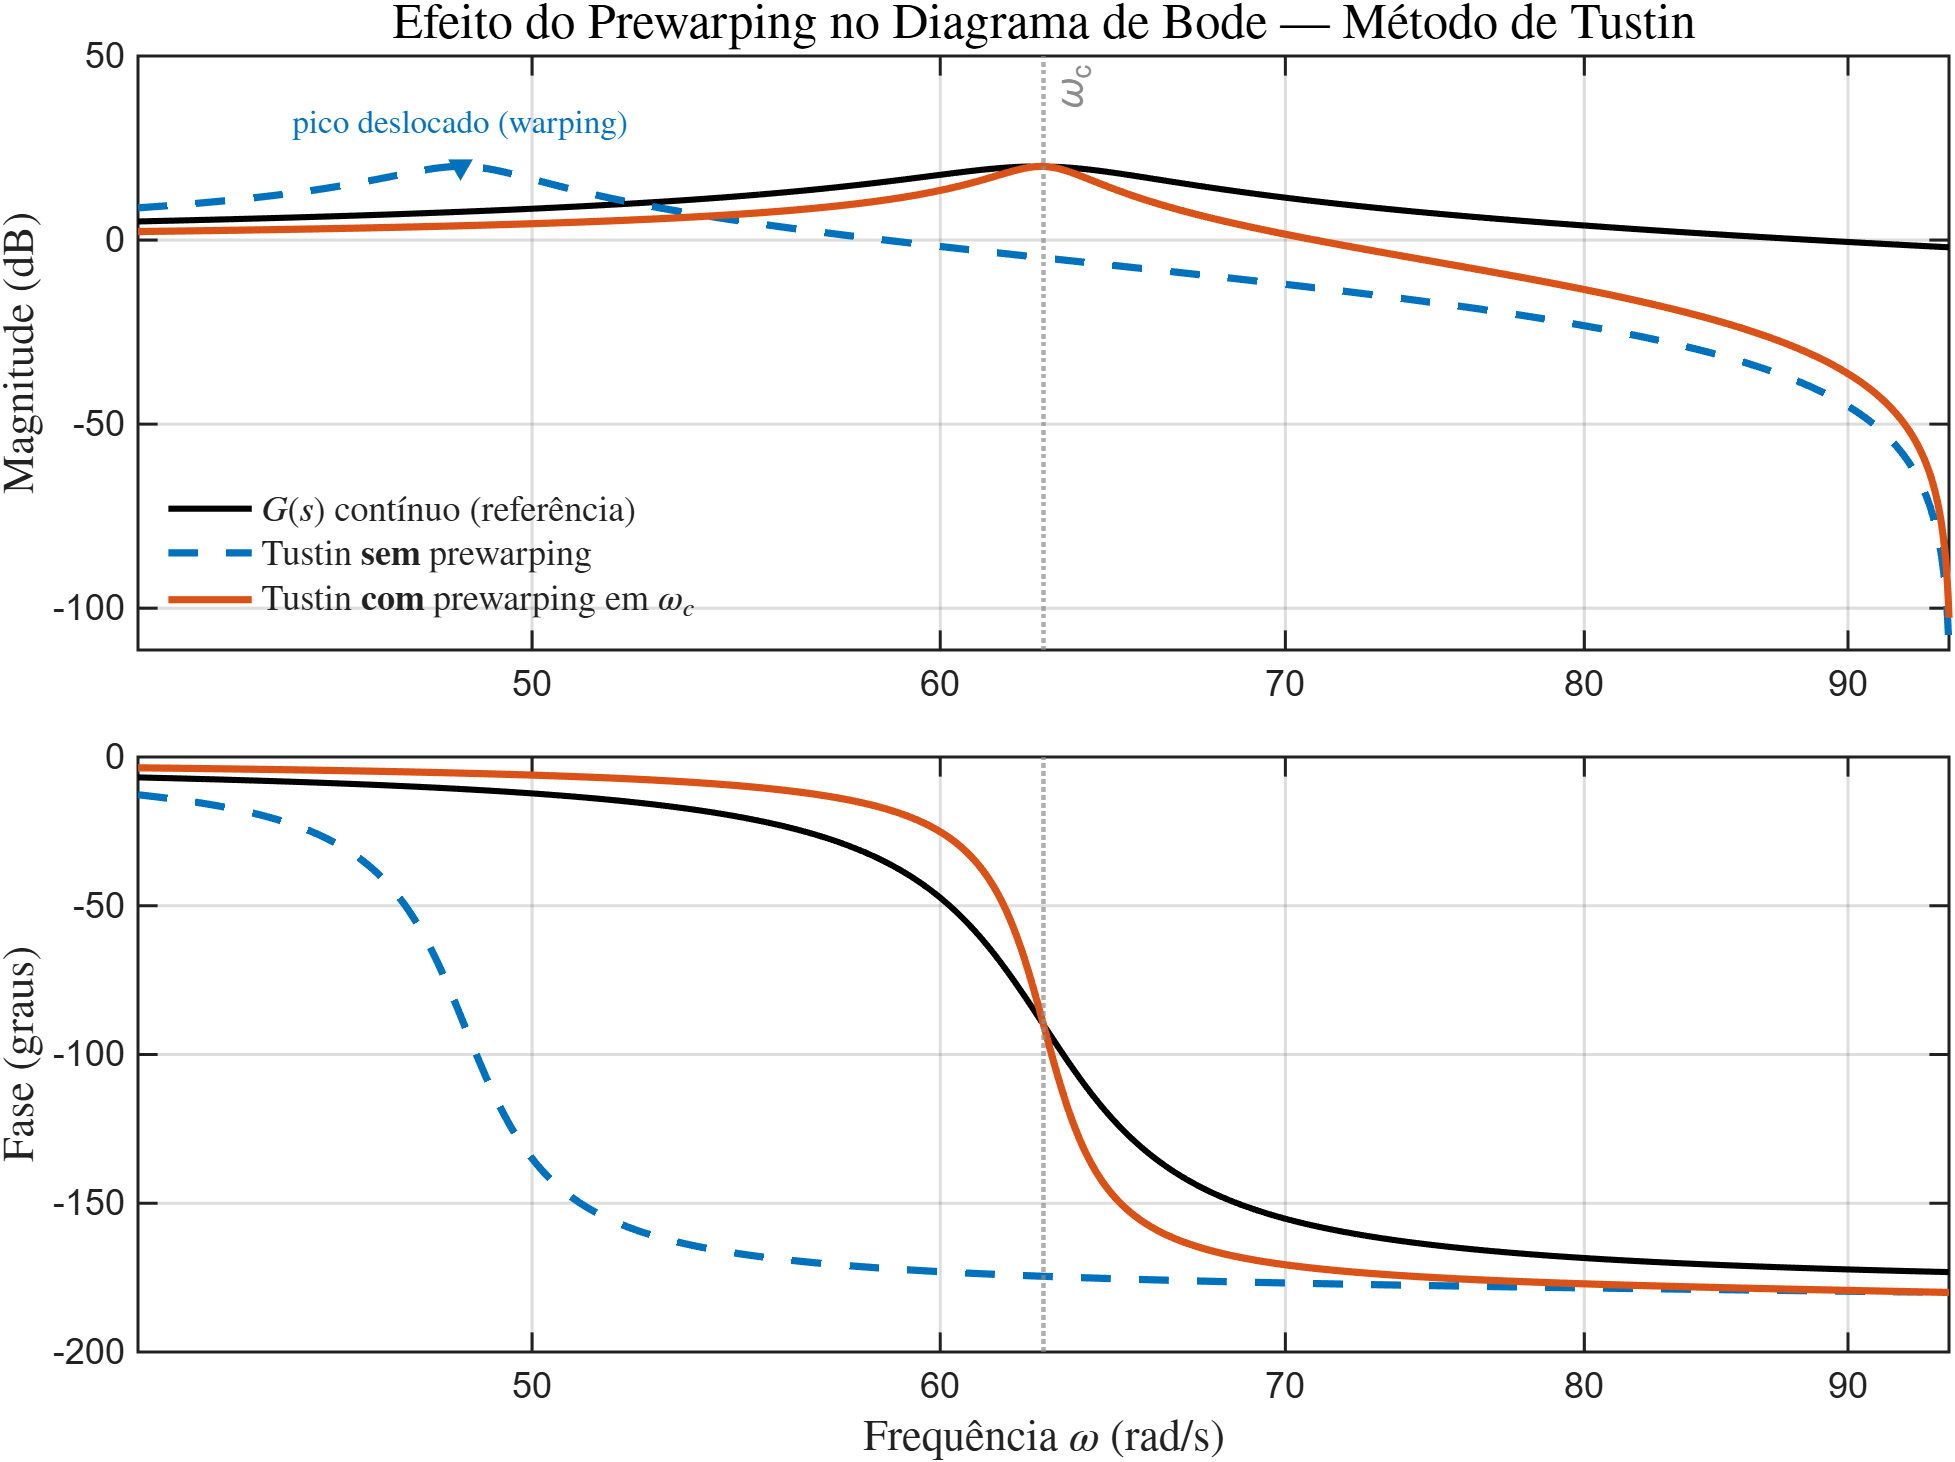
\includegraphics[width=0.62\linewidth]{bode_prewarping_tustin.png}
    \caption[Efeito do \emph{prewarping}]{Diagrama de Bode comparando a
    discretização por Tustin com e sem \emph{prewarping}. Com \emph{prewarping}, a
    resposta discreta coincide com a contínua exatamente na frequência escolhida
    $\omega_c$.}
    \label{fig:prewarp}
\end{figure}

\section{Critério de Jury}
\label{sec:jury}

Determinar a estabilidade pela Definição~\ref{def:estavel} exige conhecer as
raízes de $Q(z)$ --- tarefa impraticável à mão para graus elevados. O
\textbf{critério de Jury} decide se todas as raízes estão no interior do círculo
unitário \emph{sem calculá-las}. Ele é o análogo, em tempo discreto, do critério
de Routh--Hurwitz do tempo contínuo.

\begin{figure}[H]
    \centering
    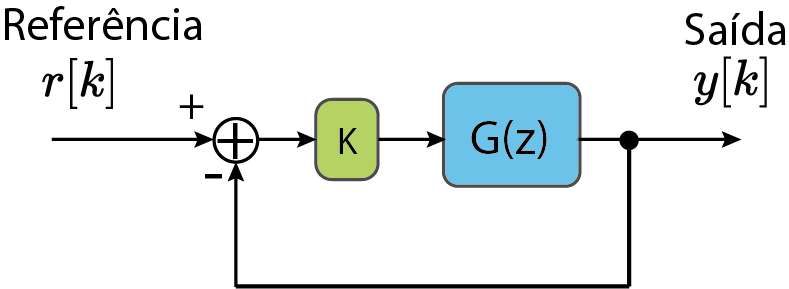
\includegraphics[width=0.62\linewidth]{malha_controle_estabilidade_z.png}
    \caption[Estabilidade sem calcular raízes]{Malha de controle discreta. A
    questão é decidir se as raízes de $Q(z)$ estão no círculo unitário sem
    resolvê-la explicitamente --- exatamente o que o critério de Jury permite.}
    \label{fig:jury_malha}
\end{figure}

\subsection{A tabela de Jury}

Seja a equação característica
\begin{empheq}[box=\tcbhighmath]{equation}
    Q(z)=a_0 z^n+a_1 z^{n-1}+\cdots+a_{n-1}z+a_n,\qquad a_0>0.
    \label{eq:Qz}
\end{empheq}

\begin{definicao}[Tabela de Jury]
\label{def:tabela}
A \textbf{tabela de Jury} é construída segundo as regras:
\begin{itemize}[nosep]
    \item a primeira linha é formada pelos coeficientes de \eqref{eq:Qz} na
    ordem decrescente de potências (de $a_0$ a $a_n$);
    \item cada linha par repete a linha ímpar imediatamente acima, na ordem
    inversa;
    \item a cada duas linhas, o número de elementos diminui em um, até a última
    linha, que possui três elementos;
    \item os coeficientes $b_k,c_k,\ldots$ são calculados pelos determinantes
    \begin{equation}
    \begin{aligned}
        b_k&=\begin{vmatrix}a_n & a_{n-1-k}\\ a_0 & a_{k+1}\end{vmatrix},
        \quad k=0,\ldots,n-1,\\
        c_k&=\begin{vmatrix}b_{n-1} & b_{n-2-k}\\ b_0 & b_{k+1}\end{vmatrix},
        \quad k=0,\ldots,n-2,\\
        &\ \vdots\\
        q_k&=\begin{vmatrix}p_3 & p_{2-k}\\ p_0 & p_{k+1}\end{vmatrix},
        \quad k=0,1,2.
    \end{aligned}
    \label{eq:jury_det}
    \end{equation}
\end{itemize}
\end{definicao}

\begin{figure}[H]
    \centering
    
\includegraphics[width=0.72\linewidth]{tabela_jury.png}
    \caption[Estrutura da tabela de Jury]{Estrutura geral da tabela de Jury para
    a equação característica $Q(z)=a_0z^n+\cdots+a_n$.}
    \label{fig:tab_jury}
\end{figure}

\subsection{Condições de estabilidade}

\begin{teorema}[Critério de Jury]
\label{teo:jury}
Considere $Q(z)$ como em \eqref{eq:Qz} com $a_0>0$.
\begin{itemize}
    \item \textbf{Sistemas de ordem $n\le 2$:} todas as raízes estão no interior
    do círculo unitário se e somente se
    \begin{equation}
        |a_n|<a_0,\qquad Q(1)>0,\qquad (-1)^n Q(-1)>0.
        \label{eq:jury2}
    \end{equation}
    \item \textbf{Sistemas de ordem $n>2$:} além das condições
    \eqref{eq:jury2}, é necessário ainda
    \begin{equation}
        |b_{n-1}|>|b_0|,\quad |c_{n-2}|>|c_0|,\quad\ldots,\quad |q_2|>|q_0|,
        \label{eq:juryn}
    \end{equation}
    isto é, $n-1$ desigualdades sobre os elementos das linhas ímpares da tabela.
\end{itemize}
\end{teorema}

\begin{figure}[H]
    \centering
    \begin{subfigure}{0.49\linewidth}
        \centering
\includegraphics[width=\linewidth]{tabela_jury2.png}
        \caption{Determinantes das primeiras linhas.}
    \end{subfigure}\hfill
    \begin{subfigure}{0.49\linewidth}
        \centering
\includegraphics[width=\linewidth]{tabela_jury3.png}
        \caption{Progressão até a última linha.}
    \end{subfigure}
    \caption[Cálculo dos coeficientes de Jury]{Cálculo sucessivo dos coeficientes
    $b_k,c_k,\ldots$ da tabela de Jury pelos determinantes $2\times2$ de
    \eqref{eq:jury_det}.}
    \label{fig:tab_jury23}
\end{figure}

\subsection{Exemplo de ordem elevada}

\begin{exemplo}[Aplicação direta do critério]
\label{ex:jury1}
Verifique se o sistema de equação característica
\begin{equation}
    Q(z)=z^4-1{,}2z^3+0{,}07z^2+0{,}3z-0{,}08=0
\end{equation}
é estável.
\end{exemplo}

\noindent\textbf{Solução.} Aqui $n=4$ e
$a_0=1,\ a_1=-1{,}2,\ a_2=0{,}07,\ a_3=0{,}3,\ a_4=-0{,}08$.

\emph{Condições \eqref{eq:jury2}:}
\begin{align*}
|a_4|=0{,}08&<a_0=1 &&\checkmark\\
Q(1)&=1-1{,}2+0{,}07+0{,}3-0{,}08=0{,}09>0 &&\checkmark\\
(-1)^4Q(-1)&=1+1{,}2+0{,}07-0{,}3-0{,}08=1{,}89>0 &&\checkmark
\end{align*}

\emph{Condições adicionais \eqref{eq:juryn} (pois $n=4>2$).} Calculam-se os
$b_k$ por \eqref{eq:jury_det}, $b_k=a_n a_{k+1}-a_{n-1-k}a_0$:
\[
b_0=-0{,}204,\quad b_1=-0{,}0756,\quad b_2=1{,}176,\quad b_3=-0{,}9936.
\]
Primeira desigualdade: $|b_3|=0{,}9936>|b_0|=0{,}204$ \checkmark. Em seguida,
$c_k=b_{n-1}b_{k+1}-b_{n-2-k}b_0$:
\[
c_0=0{,}3150,\quad c_1=-1{,}1839,\quad c_2=0{,}9456,
\]
e $|c_2|=0{,}9456>|c_0|=0{,}3150$ \checkmark. Todas as condições são satisfeitas.

\begin{destaque}
O sistema é \textbf{estável}. De fato, as raízes de $Q(z)$ são
$z\in\{0{,}8,\ 0{,}5,\ 0{,}4,\ -0{,}5\}$, todas com módulo menor que $1$ ---
confirmando o veredito do critério de Jury sem que fosse necessário calculá-las
para decidir.
\end{destaque}

\subsection{Exemplo com parâmetro de ganho}

\begin{exemplo}[Faixa de ganho estabilizante]
\label{ex:jury2}
Considere a função de transferência de malha aberta
\begin{equation}
    G(z)=\frac{K\,(0{,}3679z+0{,}2642)}{(z-0{,}3679)(z-1)}.
\end{equation}
Para quais valores de $K$ o sistema em malha fechada (realimentação unitária) é
estável?
\end{exemplo}

\noindent\textbf{Solução.} A equação característica é $Q(z)=1+G(z)=0$, ou seja,
$(z-0{,}3679)(z-1)+K(0{,}3679z+0{,}2642)=0$. Expandindo $(z-0{,}3679)(z-1)=
z^2-1{,}3679z+0{,}3679$,
\[
Q(z)=z^2+\big(-1{,}3679+0{,}3679K\big)z+\big(0{,}3679+0{,}2642K\big).
\]
Trata-se de $n=2$, com $a_0=1$, $a_1=-1{,}3679+0{,}3679K$ e
$a_2=0{,}3679+0{,}2642K$. Aplicam-se as condições \eqref{eq:jury2}:

\emph{(i)} $|a_2|<a_0$:
\[
|0{,}3679+0{,}2642K|<1
\;\Longrightarrow\;
-5{,}18<K<2{,}39.
\]

\emph{(ii)} $Q(1)>0$:
\[
Q(1)=1+(-1{,}3679+0{,}3679K)+(0{,}3679+0{,}2642K)=0{,}6321K>0
\;\Longrightarrow\; K>0.
\]

\emph{(iii)} $(-1)^2Q(-1)=Q(-1)>0$:
\[
Q(-1)=1-(-1{,}3679+0{,}3679K)+(0{,}3679+0{,}2642K)=2{,}7358-0{,}1037K>0
\;\Longrightarrow\; K<26{,}4.
\]

A interseção das três condições é dominada pelo limite superior de (i).

\begin{destaque}
O sistema em malha fechada é estável para
\[
0<K<2{,}39.
\]
Verificação: em $K=2{,}39$ os polos têm módulo unitário (limiar de
estabilidade); para $K=2{,}4$ eles saem do círculo unitário e o sistema torna-se
instável.
\end{destaque}

\section{Mapeamento bilinear no plano \texorpdfstring{$w$}{w}}
\label{sec:wplane}

Uma alternativa ao critério de Jury é transportar o problema de volta a um
domínio em que valha o critério de Routh--Hurwitz. Isso se consegue com a
transformação bilinear.

\begin{definicao}[Transformação bilinear $z\leftrightarrow w$]
Define-se a transformação bilinear
\begin{equation}
    z=\frac{1+\frac{T}{2}w}{1-\frac{T}{2}w},
    \qquad\text{equivalentemente}\qquad
    w=\frac{2}{T}\frac{z-1}{z+1}.
    \label{eq:wmap}
\end{equation}
\end{definicao}

\begin{proposicao}[A bilinear leva o disco unitário no SPE]
\label{prop:w}
A transformação \eqref{eq:wmap} mapeia o interior do círculo unitário do plano
$z$ ($|z|<1$) no semiplano esquerdo do plano $w$ ($\Real\{w\}<0$).
\end{proposicao}

\begin{proof}
A transformação \eqref{eq:wmap} tem a mesma forma da relação de Tustin
(Teorema~\ref{teo:tustin}) com os papéis de $s$ e $w$ idênticos. Pelo mesmo
cálculo daquela demonstração, $\Real\{w\}<0\iff|z|<1$. Portanto, o interior do
disco unitário corresponde exatamente ao semiplano esquerdo do plano $w$.
\end{proof}

\begin{figure}[H]
    \centering
    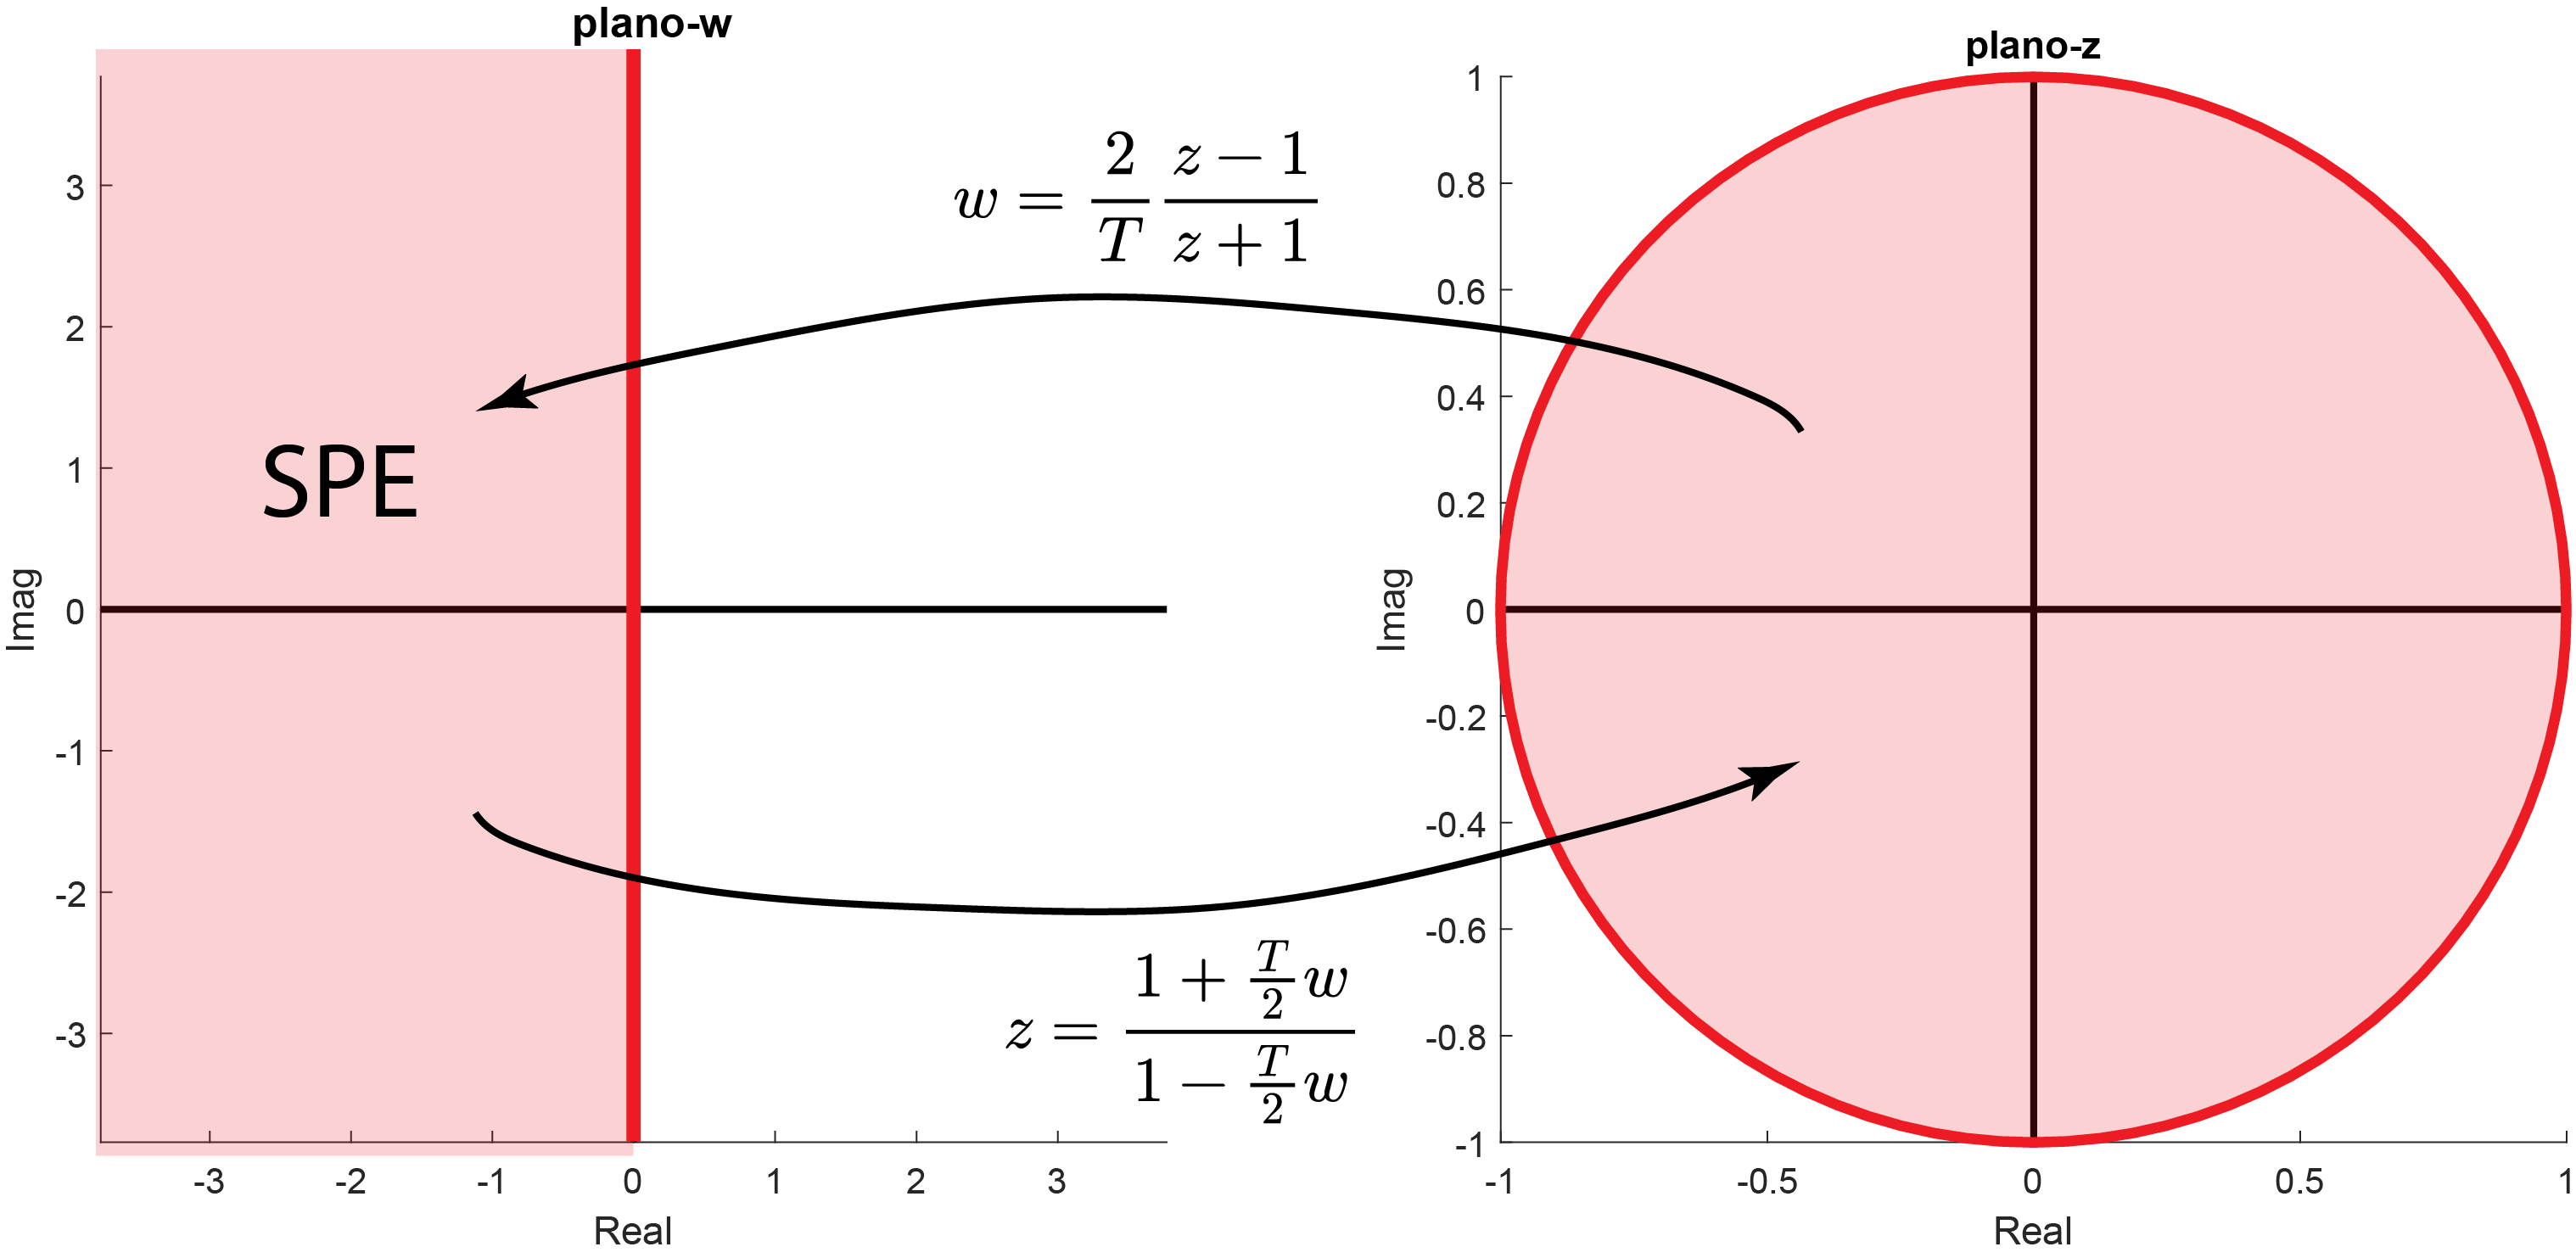
\includegraphics[width=0.75\linewidth]{map_plano_w.png}
    \caption[Plano $w$]{Mapeamento bilinear entre o plano $z$ e o plano $w$. O
    interior do círculo unitário (região estável em $z$) corresponde ao semiplano
    esquerdo em $w$, restaurando a geometria familiar do tempo contínuo.}
    \label{fig:wplane}
\end{figure}

\begin{corolario}[Estabilidade via Routh--Hurwitz]
Substituindo \eqref{eq:wmap} na equação característica $Q(z)=0$, obtém-se um
polinômio em $w$:
\begin{equation}
    Q(w)=Q(z)\Big|_{z=\frac{1+\frac{T}{2}w}{1-\frac{T}{2}w}}.
\end{equation}
Pela Proposição~\ref{prop:w}, o sistema discreto é estável se e somente se todas
as raízes de $Q(w)$ estão no semiplano esquerdo --- condição que se verifica
diretamente pelo \textbf{critério de Routh--Hurwitz}.
\end{corolario}

\section*{Síntese do capítulo}
\addcontentsline{toc}{section}{Síntese do capítulo}

Este capítulo estabeleceu o arcabouço para a análise de estabilidade em tempo
discreto. Partindo da amostragem, deduzimos a \textbf{transformada $z$}
(Definição~\ref{def:z}) e a mudança de variável $z=e^{sT}$, e demonstramos suas
propriedades essenciais --- a série geométrica (Lema~\ref{lema:geom}) e a
propriedade do deslocamento (Proposição~\ref{prop:shift}), que conecta equações a
diferenças a funções de transferência. O \textbf{mapeamento $s\to z$} foi
analisado em detalhe, culminando no Teorema~\ref{teo:regiao}: o semiplano
esquerdo mapeia-se no interior do círculo unitário, o que fixa a
\textbf{região de estabilidade discreta} (Definição~\ref{def:estavel}). Estudamos
o \textbf{efeito da discretização}, mostrando que Euler \emph{forward}
(Proposição~\ref{prop:forward}), Euler \emph{backward}
(Proposição~\ref{prop:backward}) e Tustin (Teorema~\ref{teo:tustin}) deformam a
região de estabilidade de maneiras distintas --- apenas Tustin a preserva
exatamente, ao custo da \textbf{distorção de frequência}
(Teorema~\ref{teo:warp}), corrigível por \emph{prewarping}. Por fim,
apresentamos dois métodos para decidir estabilidade sem calcular raízes: o
\textbf{critério de Jury} (Teorema~\ref{teo:jury}), aplicado a dois exemplos
completos, e o \textbf{mapeamento bilinear no plano $w$}
(Proposição~\ref{prop:w}), que devolve o problema ao critério de Routh--Hurwitz.

\begin{figure}[H]
    \centering
    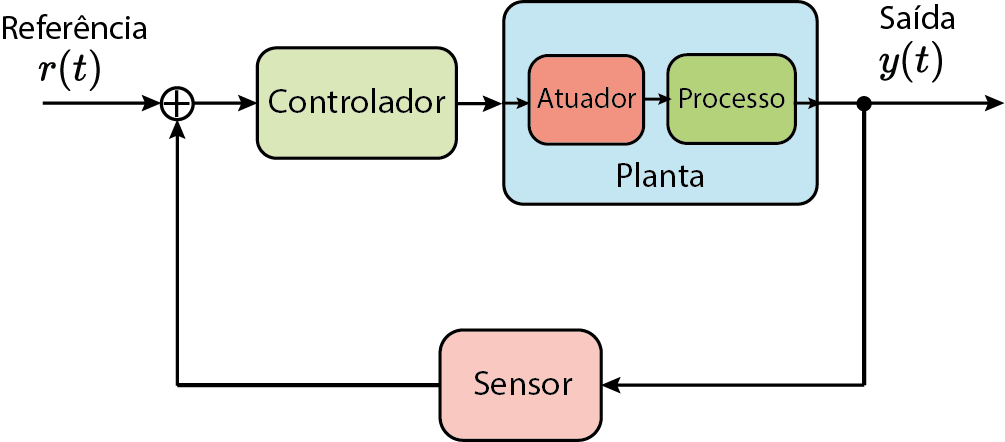
\includegraphics[width=0.72\linewidth]{malha_controle_atuador_processo.png}
    \caption[Próximos passos]{Na próxima aula (Projeto de Controladores)
    passa-se da \emph{análise} à \emph{síntese}: como projetar o controlador que
    posiciona os polos de malha fechada na região estável do plano $z$ segundo os
    critérios de desempenho desejados.}
    \label{fig:proxima}
\end{figure}

\end{document}
